\documentclass[a4paper]{article}
\usepackage[utf8]{inputenc}
\usepackage[T2A]{fontenc}
\usepackage[12pt]{extsizes}
\usepackage[normalem]{ulem}
\usepackage{calligra}
\usepackage{pdfpages}

\usepackage[english,russian]{babel}
\usepackage[left=10mm, top=10mm, right=10mm, bottom=20mm, nohead, nofoot]{geometry}
\usepackage{amsmath,amsfonts,amssymb} % математический пакет
\headsep=10mm

\usepackage[most]{tcolorbox} % для управления цветом
% НАСТРОЙКИ
%теорема
\definecolor{theorem-color}{gray}{0.90} % уровень прозрачности (1 - максимум)
\newtcolorbox{htheorem}{colback=theorem-color,grow to right by=-4mm,grow to left by=-4mm,
    boxrule=0pt,boxsep=0pt,breakable} % настройки области с изменённым фоном

%определение
\definecolor{def-color}{gray}{0.98}
\newtcolorbox{definit}{colback=def-color,grow to right by=-4mm,grow to left by=-4mm,
    boxrule=0pt,boxsep=0pt,breakable} % настройки области с изменённым фоном

%доказательсвто теоремы
\definecolor{proof-color}{gray}{0.95} % уровень прозрачности (1 - максимум)
\newtcolorbox{hproof}{colback=proof-color,grow to right by=-1mm,grow to left by=-1mm,
    boxrule=0pt,boxsep=0pt,breakable} % настройки области с изменённым фоном

%замечания, следствия
\definecolor{consectary-color}{gray}{0.95} % уровень прозрачности (1 - максимум)
\newtcolorbox{cns}{colback=consectary-color,grow to right by=-4mm,grow to left by=-4mm,
    boxrule=0pt,boxsep=0pt,breakable} % настройки области с изменённым фоном

\everymath{\displaystyle}


\usepackage{fancybox,fancyhdr}
\pagestyle{fancy}
\fancyhf{}
\fancyhead[R]{ФТ-104}
\fancyfoot[R]{\thepage}
\fancyhead[L]{колок матан 2 семестр}

\usepackage{hyperref}
\hypersetup{colorlinks=true, allcolors=[RGB]{010 090 200}} % цвет ссылок 
\newcommand{\lr}[1]{\left({#1}\right)} % команда для скобок

\title{Конспектик к коллоквиуму по матанализу}
\author{Васильев Павел}
%\linespread{1}
\usepackage{amsmath}

\usepackage{graphicx}
\usepackage{ifpdf}
\ifpdf
\DeclareGraphicsRule{*}{mps}{*}{}
\fi
\usepackage{graphicx}
\usepackage{color}
\graphicspath{ {images/} }

%\renewcommand{\familydefault}{\sfdefault}

\begin{document}

\section*{HOW TO заботать коллоквиум по матанализу (2 семестр)}


\subsection*{Список билетов}
\begin{enumerate}
\item \hyperlink{p1}{\sout{Понятие определённого интеграла}}
\item \hyperlink{p2}{\sout{Интегрируемость суммы функций}}
\item \hyperlink{p3}{\sout{Ограниченность интегрируемой функции}}
\item \hyperlink{p4}{\sout{Пример ограниченной неинтегрируемой функции}}
\item \hyperlink{p5}{\sout{Суммы Дарбу и их свойства}}. Критерий интегрируемости
\item \hyperlink{p6}{\sout{Аддитивность интеграла по множеству}}
\item \hyperlink{p7}{\sout{Интегрируемость непрерывной функции}}
\item \hyperlink{p8}{\sout{Интегрируемость монотонной функции}}
\item \hyperlink{p9}{\sout{Неизменность интеграла при изменении функции в конечном числе точек}}
\item \hyperlink{p10}{\sout{Интегрируемость композиции непрерывной и интегрируемой функций}}
\item \hyperlink{p11}{\sout{Интегрируемость произведения функций}}
\item \hyperlink{p12}{\sout{Интеграл с переменным верхним пределом: непрерывность и дифференцируемость}}
\item \hyperlink{p13}{Формула Ньютона-Лейбница}
\item \hyperlink{p14}{\sout{Пример неинтегрируемой функции с первообразной}}
\item \hyperlink{p15}{\sout{Пример интегрируемой функции без первообразной}}
\item \hyperlink{p16}{\sout{Интегрирование по частям}}
\item \hyperlink{p17}{\sout{Замена переменной}}
\item \hyperlink{p18}{\sout{Первая теорема о среднем}}
\item Вычисление площадей - \textbf{что здесь писать, друзья?}
\item \hyperlink{p20}{\sout{Вычисление длины дуги}}
\item\hyperlink{p21}{\sout{Приближённое вычисление интеграла: методы прямоугольников, трапеций, Симпсона}}
\end{enumerate}

\subsection*{\hyperlink{tasks}{Несколько задач для подготовки с решением}}

\newpage

\begin{definit}
\hypertarget{p1}{}
\subsection*{Понятие определённого интеграла}

\textit{Разбиение} отрезка $[a, b]$ - $\{ a = x_0, x_1, ..., x_n = b\}$, $x_i < x_{i+1}$

\textit{Мелкость} разбиения: $$\lambda = \max_{1 \leq k \leq n} \Delta x_k = \max (x_k - x_{k-1})$$

\textit{Интегральная сумма}: $S(f, \tau, \xi) = \sum_{k=1}^n f(\xi_k) \Delta x_k = S_\tau$

\textbf{Определение} $f$, определённая на $[a,b]$, интегрируема по Риману на $[a,b]$, если

$$\exists I \in \mathbb{R}: \quad \forall \varepsilon > 0 \exists \delta (\varepsilon) \quad \forall \tau  \forall \xi \quad (\lambda_t < \delta \Rightarrow |S(f, \tau, \xi) - I| < \varepsilon)$$

Обозначаем $I = \int_a^b f(x)dx$


\end{definit}

\begin{definit}
\hypertarget{p2}{}
\subsection*{Интегрируемость суммы функций}
\begin{htheorem}\textbf{Теорема}.
Пусть $f$ и $g$ интегрируемы на $[a,b]$ и $\alpha, \beta \in \mathbb{R}$. Тогда $\alpha f + \beta g$ интегрируема на $[a,b]$ и $$\int_a^b(\alpha f + \beta g)dx = \alpha \int_a^b fdx + \beta \int_a^b gdx$$
\end{htheorem}

\begin{hproof}\textbf{Доказательство.}
$$S(\alpha f + \beta g, \tau, \xi) = \sum_{k=1}^n (\alpha f(\xi_k) + \beta g(\xi_k)) \Delta x_k = \newline \alpha \sum_{k=1}^n f(\xi_k) \Delta x_k + \beta \sum_{k=1}^n g(\xi_k) \Delta x_k = $$ 

$$= \alpha S(f, \tau, \xi) + \beta S(g, \tau, \xi)$$


$$ \left| S(\alpha f + \beta g, \tau, \xi) - \left( \alpha \int_a^b fdx + \beta \int_a^b gdx \right) \right| \leq |\alpha| \left| S(f, \tau, \xi) - \int_a^b f \right| + |\beta| \left| S(g, \tau, \xi) - \int_a^b g  \right|$$

В определении интегрируемости $f$ и $g$ берём не $\varepsilon$, а $\frac{\varepsilon}{|\alpha|+|\beta|}$

Тогда $$ \left| S(f, \tau, \xi) - \int_a^b f \right| \leq \frac{\varepsilon}{|\alpha|+|\beta|}\quad \text{и} \quad \left| S(g, \tau, \xi) - \int_a^b g  \right| \leq \frac{\varepsilon}{|\alpha|+|\beta|} \Rightarrow$$

$$
\Rightarrow |\alpha| \left| S(f, \tau, \xi) - \int_a^b f \right| + |\beta| \left| S(g, \tau, \xi) - \int_a^b g  \right| < \varepsilon$$

\end{hproof}
\end{definit}

\begin{definit}
\hypertarget{p3}{}
\subsection*{Ограниченность интегрируемой функции}

\begin{htheorem}\textbf{Теорема}.
Если $f$ интегрируема на $[a,b]$, то она ограничена на $[a,b]$.

\end{htheorem}

\begin{hproof}\textbf{Доказательство.}

Проведём от противного: пусть $f$ не ограничена, но интегрируема.

Тогда $I - \varepsilon < \sum_{k=1}^n f(\xi_k) \Delta x_k < I + \varepsilon$ для какого-то разбиения $\tau$ при заданном $\varepsilon > 0$ и любом выборе $\xi_k \in [x_{k-1}, x_k]$.

Так как $f$ не ограничена, то найдётся такой отрезок $[x_{k-1}, x_k]$, на котором $f$ не ограничена $\Rightarrow \sum_{k=1}^n f(\xi_k) \Delta x_k $ можно сделать сколь угодно большим по модулю. Противоречие.
\end{hproof}

\end{definit}


\begin{definit}
\hypertarget{p4}{}
\subsection*{Пример ограниченной неинтегрируемой функции}

Например, функция Дирихле $D(x)$:

\[
	D(x) = \begin{cases}
		1, x \in \mathbb{Q} \\
		0, x \notin \mathbb{Q}
	\end{cases}
\]

\[
	\forall x \in [a,b] \quad D(x) \quad \text{не интегрируема на} \quad  [a, b], \quad \text{так как}
\]

\begin{enumerate}
\item $\{ \xi_k \} \subset \mathbb{R} \backslash \mathbb{Q}, f(\xi_k) = 0 \Rightarrow \forall \tau S_\tau = 0$
\item $\{ \xi_k \} \subset \mathbb{Q}, f(\xi_k) = 1 \Rightarrow \forall \tau S_\tau = \sum \Delta x_k = b - a$
\end{enumerate}
\end{definit}


\begin{definit}
\hypertarget{p5}{}
\subsection*{Суммы Дарбу и их свойства. Критерий интегрируемости.}
В 100 раз лучше описано \href{https://univerlib.com/mathematical_analysis/definite_integral/definite_integral_def/}{здесь}

Пусть $f$, определённая на $[a,b]$, ограничена на этом отрезке и пусть $\tau = \{ x_0, ..., x_n\}$ - разбиение отрезка $[a,b]$.

\[
M_i = \sup_{x \in [x_{i-1}, x_i]} f(x), m_i = \inf_{x \in [x_{i-1}, x_i]} f(x)
\]

\[
\overline{S_\tau} = \sum_{i=1}^n M_i \Delta x_i, \underline{S_\tau} = \sum_{i=1}^n m_i \Delta x_i
\]

Это верхняя и нижняя суммы Дарбу соответственно.

\begin{enumerate}
\item Для любой выборки точек $\xi_i$ справедливо 

\[
\underline{S_\tau} \leq S_\tau \leq \overline{S_\tau}  
\]

\textbf{Доказательство.}

Так как для любого $\xi_i \in [x_{i-1}, x_i]$: 
\[
m_i \leq f(\xi_i) \leq M_i
\]

то

\[
m_i \Delta x_i \leq f(\xi_i) \Delta x_i \leq M_i \Delta x_i
\]

Складывая эти неравенства, получаем

\[
\sum_{i=1}^n m_i \Delta x_i \leq \sum_{i=1}^n f(\xi_i) \Delta x_i \leq \sum_{i=1}^n M_i \Delta x_i
\]

Это в точности то, что нужно было доказать.

\item \[\overline{S_\tau} = \sup_{\xi} S_\tau(\xi)\]

\[\underline{S_\tau} = \inf_{\xi} S_\tau(\xi)\]

\textbf{Доказательство.}
\begin{enumerate}
\item \[\overline{S_\tau} = \sup_{\xi} S_\tau(\xi)\]

Согласно определению точной верхней грани, нужно доказать, что выполняются следующие условия:
\[
\begin{cases}
\forall \xi \rightarrow S_\tau \leq \overline{S_\tau} \\ \forall \varepsilon > 0 \exists \xi': \overline{S_\tau} - S_\tau < \varepsilon
\end{cases}
\]

Первое из этих условий выполняется очевидно по первому свойству. Докажем второе условие. Так как $M_i = \sup_{x \in [x_{i-1}, x_i]} f(x)$, то по определению точной верхней грани 
\[
\forall \varepsilon \quad \exists \xi_i'(\varepsilon) \in [x_{i-1}, x_i]: 0 \leq M_i - f(\xi_i') \leq \frac{\varepsilon}{b-a}
\]

Домножим $i$-е неравенство на $\Delta x_i$ и складывая все неравенства
\[
0 \leq \overline{S_\tau} - S_\tau < \varepsilon
\]

\item \[\underline{S_\tau} = \inf_{\xi} S_\tau(\xi)\] аналогично.
\end{enumerate}

\item Если разбиение $\tau_2$ - измельчение разбиения $\tau_1$, то 
\[
\underline{S_{\tau_1}} \leq \underline{S_{\tau_2}} \leq \overline{S_{\tau_2}} \leq \overline{S_{\tau_1}}
\]
То есть при измельчении разбиения нижняя сумма Дарбу не уменьшается, а верхняя не увеличивается.

\textbf{Доказательство.} Для доказательства достаточно рассмотреть случай, когда $\tau_2$ получается из $\tau_1$ путём добавления только одной точки $x' \in (x_{i-1}, x_i)$.

\[ \Delta x_i = [x_{i-1}, x'] + [x', x_i] \]

Пусть $m_i' = \inf_{x \in [x_{i-1}, x']} f(x), m_i'' = \inf_{x \in [x', x_{i}]}$. Тогда очевидно $m_i' \geq m_i, m_i'' \geq m_i$.

В суммах $\underline{S_{\tau_2}}$ и $\underline{S_{\tau_1}}$ равны все соответствующие слагаемые, кроме тех, которые связаны с отрезком $[x_{i-1}, x_i]$.

Поэтому $\underline{S_{\tau_2}} - \underline{S_{\tau_1}} = m_i'(x'-x_{i-1}) + m_i''(x_i-x') - m_i(x_i-x_{i-1})$, где $m_i' \geq m_i, m_i'' \geq m_i$.

Следовательно 

\[
\underline{S_{\tau_2}} - \underline{S_{\tau_1}} = (m_i' - m_i)(x'-x_{i-1}) + (m_i'' - m_i) (x_i-x') \geq 0
\]

то есть \[\underline{S_{\tau_1}} \leq \underline{S_{\tau_2}}\]

Аналогично и с $\overline{S_{\tau_2}} \leq \overline{S_{\tau_1}}$.

\item Для любых $\tau', \tau''$ 
\[
\underline{S_{\tau'}} \leq \overline{S_{\tau''}}
\]

\textbf{Доказательство.} Пусть $\tau$ - измельчённое разбиение и $\tau'$, и $\tau''$. Тогда $\underline{S_{\tau'}} \leq \underline{S_\tau} \leq \overline{S_\tau}.$

\[
\overline{S_\tau} \leq \overline{S_{\tau''}}
\] по предыдущему пункту, где $\tau_2 = \tau, \tau_1 = \tau'$.

Объединяя, получаем $\underline{S_{\tau'}} \leq \underline{S_\tau} \leq \overline{S_\tau} \leq \overline{S_{\tau''}}$

\item \[
\exists \underline{J} = \sup_\tau \underline{S_\tau}, \overline{J} = \inf_\tau \overline{S_\tau}
\] такие, что $\forall \tau', 
\tau'' \quad \underline{S_{\tau'}} \leq \underline{J} \leq \overline{J} \leq \overline{S_{\tau''}} $

\end{enumerate}


\end{definit}



\begin{definit}
\hypertarget{p6}{}
\subsection*{Аддитивность интеграла по множеству}

Пусть $c \in (a, b)$ и функция $f(x)$ определена и интегрируема на отрезке $[a, b]$. Тогда интеграл функции $f(x)$ на отрезке $[a, b]$ равен сумме интегралов функции $f(x)$ на отрезках $[a, c]$ и $[c, b]$:

\[
\int_{a}^{b} f(x) \, dx = \int_{a}^{c} f(x) \, dx + \int_{c}^{b} f(x) \, dx
\]

\textbf{Доказательство:}

Поскольку $f(x)$ интегрируема на отрезке $[a, b]$, для любого $\varepsilon > 0$ существует разбиение $\tau = \{a, x_1, \dots, x_{n-1}, b\}$ отрезка $[a, b]$ такое, что верхняя сумма Дарбу $\overline{S_\tau}$ и нижняя сумма Дарбу $\underline{S_\tau}$ удовлетворяют условию:

\[
\overline{S_\tau} - \underline{S_\tau} < \varepsilon
\]

Выберем такое разбиение, которое включает точку $c$. Теперь разбиваем $\tau$ на два подмножества $\tau'$ и $\tau''$, соответствующие отрезкам $[a, c]$ и $[c, b]$, так что $\tau = \{x_i \in \tau \mid x_i \leq c\}$ и $\tau'' = \{x_i \in \tau \mid x_i \geq c\}$.

Тогда верхние и нижние суммы Дарбу для $f(x)$ на отрезках $[a, c]$ и $[c, b]$ будут равны $\overline{S_{\tau'}}$ и $\underline{S_{\tau'}}$, а также $\overline{S_{\tau''}}$ и $\underline{S_{\tau'}}$ соответственно.

Поскольку разбиение $\tau$ является объединением $\tau'$ и $\tau''$, имеем:

\[
\overline{S_{\tau}} \geq \overline{S_{\tau'}} + \overline{S_{\tau''}}
\]
\[
\underline{S_{\tau}} \leq \underline{S_{\tau'}} + \underline{S_{\tau''}}
\]

Из этого следует, что:

\[
(\overline{S_{\tau'}} + \overline{S_{\tau''}} )- (\underline{S_{\tau'}} + \underline{S_{\tau''}}) < \varepsilon
\]

\[
(\overline{S_{\tau'}} - \underline{S_{\tau'}}) + (\overline{S_{\tau''}} - \underline{S_{\tau''}}) < \varepsilon
\]

\[
\overline{S_{\tau'}} - \underline{S_{\tau'}} < \varepsilon
\]

\[
\overline{S_{\tau''}} - \underline{S_{\tau''}} < \varepsilon
\]

Пусть $f$ интегрируема на $[a,c]$ и $[c,b]$. Тогда $\exists \int_a^b f$.

\[
\overline{S_\tau} = \sum_{k \neq j} + M_j \Delta x_j
\]

\[
\underline{S_\tau} = \sum_{k \neq j} + m_j \Delta x_j
\]

Хотим получить $\overline{S_\tau} \leq \overline{S_{\tau'}} + \overline{S_{\tau''}} + \text{что-то}$

\[
\overline{S_\tau} - (\overline{S_{\tau'}} + \overline{S_{\tau''}}) \leq \text{что-то}
\]

\[
\overline{S_\tau} - (\overline{S_{\tau'}} + \overline{S_{\tau''}}) = M_j \Delta x_j - \left( \sup_{[x_{j-1}, c]} f(x) \right) (c-x_{j-1}) + \left( \sup_{[c, x_j]} f(x) \right)(x_j-c) \leq
\]

\[
\leq B \Delta x_j + B (c-x_{j-1} + x_j -c) = 2B \Delta x_j \leq 2B \lambda_\tau
\] 

\[\overline{S_\tau} - (\overline{S_{\tau'}} + \overline{S_{\tau''}}) \leq 2B \lambda_\tau\]

\[\underline{S_\tau} \geq (\underline{S_{\tau'}} + \underline{S_{\tau''}}) - 2B \lambda_\tau\]

\[\overline{S_\tau} - \underline{S_\tau} \leq \overline{S_{\tau'}} + \overline{S_{\tau'}} + 2B \lambda_\tau - S_{\tau'} - S_{\tau''} = (\overline{S_{\tau'}} - \underline{S_{\tau'}}) + (\overline{S_{\tau''}} - \underline{S_{\tau''}}) + 4B\lambda_\tau < \varepsilon\]

\[
\overline{S_{\tau'}} - \underline{S_{\tau'}} < \frac{\varepsilon}{3}
\]

\[
\overline{S_{\tau''}} - \underline{S_{\tau''}} < \frac{\varepsilon}{3}
\]

так как берём минимальную дельту.

Докажем уже наконец-то, что $\displaystyle \int_a^b f = \int_a^c f + \int_c^b f $

$\displaystyle \left| \int_a^b - \left( \int_a^c + \int_c^b \right) \right| < \varepsilon$

$\displaystyle \left| \int_a^b - \left( \int_a^c + \int_c^b \right) + \left( S_{\tau'} + S_{\tau''} \right) - (S_{\tau'} + S_{\tau''}) \right| < \varepsilon$

$\displaystyle \left| \int_a^b - \left( \int_a^c + \int_c^b \right) + \left( S_{\tau'} + S_{\tau''} \right) - (S_{\tau'} + S_{\tau''}) \right| \leq \left| \int_a^b -  (S_{\tau'} + S_{\tau''}) \right| + \left| \int_a^c - S_{\tau'} \right| + \left| \int_c^b - S_{\tau''} \right| <\varepsilon$

$\left| \int_a^b - ( S_{\tau'} + S_{\tau''}) \right| < \frac{\varepsilon}{3}$

$ \left| \int_a^c - S_{\tau'} \right| < \frac{\varepsilon}{3}$

$\left| \int_c^b - S_{\tau''} \right| < \frac{\varepsilon}{3}$


\end{definit}

\begin{definit}
\hypertarget{p7}{}
\subsection*{Интегрируемость непрерывной функции}
\begin{htheorem}
\textbf{Теорема}.

Пусть $f$ непрерывна на $[a,b]$, тогда $f$ интегрируема на $[a,b]$.
\end{htheorem}


\begin{hproof}\textbf{Доказательство.}

$f$ непрерывна на $[a,b]$, значит она равномерно нерпрерывна на $[a,b]$ (теорема Кантора):

\[
\forall \varepsilon > 0 \quad \exists \delta ( \varepsilon ) \quad \forall x', x'' \in [a,b] \quad |x'-x''| < \delta \Rightarrow |f(x') - f(x'')| < \varepsilon
\]

Теперь поймём, что 

\[
\forall \varepsilon' > 0 \quad \exists \delta'(\varepsilon') > 0 \quad \forall \tau \quad (\lambda_\tau < \delta' \Rightarrow \overline{S_\tau} - \underline{S_\tau} < \varepsilon')
\]

Рассмотрим разбиение $\tau$, у которого $\lambda_\tau < \delta$ ($\delta$ берём из определения равномерной непрерывности).

\[
\overline{S_\tau} - \underline{S_\tau} = \sum_{k=1}^n (M_k-m_k) \Delta x_k
\]

\[
\forall \xi_j', \xi_j'' \in [x_j, x_{j+1}] \quad |\xi_j' - \xi_j''| < \delta, \quad \text{так как} \quad \lambda_\tau < \delta
\]

И по равномерной непрерывности получаем

\[
|f(\xi_j') - f(\xi_j'')| < \varepsilon
\]

\hypertarget{supinf}{}
\[
|f(\xi_j') - f(\xi_j'')| < \varepsilon \Leftrightarrow M_j - m_j < \varepsilon
\]

Докажем это утверждение ($sup - inf$):
\begin{enumerate}
\item $\Leftarrow$:

\[
M_j - m_j < \varepsilon
\]

\[
\begin{cases}
f(\xi_j') \leq M_j \\
f(\xi_j'') \geq m_j \\
\end{cases}
\Rightarrow f(\xi_j') - f(\xi_j'') \leq M_j-m_j < \varepsilon
\]

\item $\Rightarrow$:

Знаем $|f(\xi_j)' - f(\xi_j'')| < \varepsilon$.

Возьмём $\sup$ по $\xi_j'$:

\[
	\sup_{\xi_j'}(f(\xi_j') - f(\xi_j'')) = M_j - f(\xi_j'') \leq \varepsilon
\]

А затем возьмём $\inf$ по $\xi_j''$ и получим:

\[
M_j - m_j < \varepsilon
\]

\end{enumerate}

Мы доказали 

\[
|f(\xi_j)' - f(\xi_j'')| < \varepsilon \Leftrightarrow M_j - m_j < \varepsilon
\]

\[
\overline{S_\tau} - \underline{S_\tau} = \sum_{k=1}^n (M_k-m_k) \Delta x_k < \varepsilon \sum_{k=1}^n \Delta x_k = \varepsilon (b-a)
\]
\end{hproof}


\end{definit}


\begin{definit}
\hypertarget{p8}{}
\subsection*{Интегрируемость монотонной функции}

\begin{htheorem}\textbf{Теорема}.

Пусть $f$ монотонна на $[a,b]$. Тогда $f$ интегрируема $[a,b]$.
\end{htheorem}

\begin{hproof}\textbf{Доказательство.}

Б.о.о. скажем, что $f$ монотонно возрастает.

Определение интегрируемости:

\[
\forall \varepsilon > 0 \quad \exists \delta(\varepsilon) > 0 \quad \forall \tau \quad (\lambda_\tau < \delta \Rightarrow \overline{S_\tau} - \underline{S_\tau} < \varepsilon)
\]

\[
\overline{S_\tau} - \underline{S_\tau} = \sum_{k=1}^n (M_k-m_k) \Delta x_k = \sum_{k=1}^n (f(x_k) - f(x_{k-1})) \Delta x_k \leq \delta \sum_{k=1}^n (f(x_k) - f(x_{k-1}))
\]

\[
\delta \sum_{k=1}^n (f(x_k) - f(x_{k-1})) = \delta (f(b)-f(a))
\]

Ну и чтобы $\delta (f(b)-f(a))$ было меньше $\varepsilon$, возьмём $\delta < \frac{\varepsilon}{f(b)-f(a)}$.
\end{hproof}
\end{definit}

\begin{definit}
\hypertarget{p9}{}
\subsection*{Неизменность интеграла при изменении функции в конечном числе точек}
\begin{htheorem}\textbf{Теорема}.

Пусть $f$ интегрируема $[a,b]$. Тогда если поменяем $f$ в конечном числе точек, то площадь останется неизменной.
\end{htheorem}


\begin{hproof}\textbf{Доказательство.}

Пусть $\breve{f}$ это $f$, у которой поменяли $f(x_0)$ на $c$

\[
g(x) = \begin{cases} 0, x \neq x_0 \\ f(x_0) - c, x=x_o  \end{cases}
\]

\[
\int_a^b g(x)dx = 0
\]

\[
\forall \tau |s_\tau| \leq |c - f(x_0)| \cdot \lambda_\tau \rightarrow 0 \Rightarrow \int_a^b g(x)dx = 0
\]

\[
\int_a^b f = \int_a^b (\breve{f} + g) = \int_a^b \breve{f} + 0 =  \int_a^b \breve{f}
\]
\end{hproof}
\end{definit}

\begin{definit}
\hypertarget{p10}{}
\subsection*{Интегрируемость композиции непрерывной и интегрируемой функций}

\begin{htheorem}\textbf{Теорема}.

Пусть $f$ интегрируема на $[a,b]$ и принимает значения в $[c,d]$. Пусть $\Phi$ непрерывна на $[c,d]$. Тогда $\Phi(f(x))$ интегрируема на $[a,b]$.
\end{htheorem}

\begin{hproof}\textbf{Доказательство.}

$\Phi$ равномерно непрерывна на $[c,d]$:

\[
\forall \varepsilon > 0 \exists \delta(\varepsilon) \quad \forall x', x'' \in [c,d] \quad |x'-x''| < \delta \Rightarrow |f(x')-f(x'')|<\varepsilon
\]

Хотим $\overline{S_\tau(\Phi(f))} - \underline{S_\tau(\Phi(f))} < \varepsilon$.

$f$ интегрируема $\Rightarrow$ если $\lambda_\tau < \delta$, то 

\[
\overline{S_\tau(f)} - \underline{S_\tau(f)} < \delta^2
\]

Это мы так взяли $\varepsilon = \delta^2$.

Хотим оценить $\overline{S_\tau(\Phi(f))} - \underline{S_\tau(\Phi(f))} = \sum_{k=1}^n (M_k(\Phi(f)) - m_k(\Phi(f))) \Delta x_k$

Имеем здесь 2 семейства индексов:

\begin{enumerate}
\item $I = \{k: M_k(f) - m_k(f) < \delta \}$
\item $J = \{k: M_k(f) - m_k(f) \geq \delta \}$
\end{enumerate}


\begin{enumerate}
\item $k \in I$:

\[
f(\xi_k') - f(\xi_k'') < \delta \Rightarrow | \Phi(f(\xi')) - \Phi(f(\xi''))| < \varepsilon \Rightarrow
\]

\[
\Rightarrow \text{по лемме (\hyperlink{supinf}{$sup - inf$})} \quad M_k(\Phi(f)) - m_k(\Phi(f)) < \varepsilon
\]

\[
\sum_{k \in I} \left( M_k(\Phi(f)) - m_k(\Phi(f)) \right) \Delta x_k < \varepsilon (b-a)
\]
\item $k \in J$:
\[
\overline{S_\tau(f)} - \underline{S_\tau(f)} < \delta^2
\]

Так как для каждого $k$ $M_k(f) - m_k(f) \geq \delta$, то

\[
 \delta \sum_{k \in J} \Delta x_k \leq \overline{S_\tau(f)} - \underline{S_\tau(f)} < \delta^2
\]

\[
\sum_{k \in J} \Delta x_k \leq \delta
\]

$\Phi$ непрерывна на $[c,d] \Rightarrow$ ограничена числом $L$.

\[
\sum_{k \in J} M_k(\Phi(f)) - m_k(\Phi(f)) \Delta x_k \leq 2L \sum_{k \in J} \Delta x_k  \leq 2L\varepsilon
\]

\end{enumerate}
\end{hproof}


\end{definit}

\begin{definit}
\hypertarget{p11}{}
\subsection*{Интегрируемость произведения функций}

\begin{htheorem}\textbf{Теорема}.
Пусть $f$ и $g$ интегрируемы на $[a,b]$. Тогда $f \cdot g$ тоже интегрируема на $[a,b]$.

\end{htheorem}


\begin{hproof}\textbf{Доказательство.}
\[
(f-g)^2 = f^2 - 2fg + g^2
\]

$(f-g)^2$ интегрируема, так как $f-g$ интегрируема и $(...)^2$ интегрируемо (по интегрируемости композиции непрерывной и интегрируемой функции).

\[
fg = \frac{f^2 + g^2 - (f-g)^2}{2}
\]

Правая часть равенства интегрируема, значит левая тоже.
\end{hproof}
\end{definit}

\begin{definit}
\hypertarget{p12}{}
\subsection*{Интеграл с переменным верхним пределом: непрерывность и дифференцируемость}

\textbf{Определение.} Пусть $f$ интегрируема на $[a,b]$ $\Rightarrow \forall x \in (a,b) \quad \exists \int_a^x f(t)dt$.

$\Phi(x) = \int_a^x f(t)dt$ - интеграл с переменным верхним пределом (договоримся, что $\int_a^a = 0$).

\begin{htheorem}\textbf{Теорема}.

Пусть $f$ ограничена на $[a,b]$. Тогда $\Phi$ непрерывна и \\ $\exists C: \quad |\Phi(x) - \Phi(y)| \leq C|x-y| \quad \forall x, y \in (a,b)$ (\textit{липшицевость}).
\end{htheorem}

\begin{hproof}\textbf{Доказательство.}
Из липшицевости следует непрерывность по определению непрерывности ($\delta = \frac{\varepsilon}{C}$) (типа множество липшицевостных функций является подмножеством непрерывных функций)


Предположим $x<y$:

\[
	|\Phi(x) - \Phi(y)| = \left| \int_a^x f(t)dt - \int_a^y f(t) dt \right| = \left| \int_x^y f(t)dt \right| \leq 
\]

\[\leq \begin{bmatrix}
	\left| \sum f(\xi_k) \Delta x_k \right| \leq \sum \left| f(\xi_k) \right| \Delta x_k \Rightarrow \\
	\Rightarrow \left| \int f \right| \leq \int |f|
	\end{bmatrix} \leq
\]
 
\[ \leq
 \begin{bmatrix}
 |f| \leq B
 \end{bmatrix} \leq B \cdot \left| \int_x^y dt \right| \leq B(y-x)
\]
\end{hproof}

\begin{htheorem}\textbf{Теорема}.

Пусть $f$ непрерывна на $[a,b]$. Тогда $\forall x_0 \in (a,b) \quad \Phi'(x_0) = f(x_0)$.
\end{htheorem}

\begin{hproof}\textbf{Доказательство.}

\[
\Phi'(x) = \lim_{h \rightarrow 0} \frac{\Phi(x_0 + h) - \Phi(x_0)}{h}
\]

\[
 \frac{\Phi(x_0 + h) - \Phi(x_0)}{h} = \frac{\int_{x_0}^{x_0+h} f(t)dt}{h} = \frac{\int_{x_0}^{x_0+h} f(t)dt - f(x_0)h}{h} + f(x_0) = 
\]

\[
 = \frac{\int_{x_0}^{x_0+h} (f(t) - f(x_0))dt}{h} + f(x_0)
\]
\[
\left|  \frac{\Phi(x_0 + h) - \Phi(x_0)}{h} - f(x_0) \right| = \left| \frac{\int_{x_0}^{x_0+h} (f(t) - f(x_0))dt}{h} \right| \leq \frac{1}{h} \int_{x_0}^{x_0+h} |f(t) - f(x_0)|dt
\]

О, а ведь $f$ непрерывна: 
\[
\forall \varepsilon > 0 \exists \delta: 0<|t-x_0|<\delta \Rightarrow |f(t) - f(x_0)| < \varepsilon
\]

Тут мы берём любой $\varepsilon$, по нему находим $\delta$ и берём $h < \delta$. Тогда $|x_0-t| < h$.


\[
\frac{1}{h} \int_{x_0}^{x_0+h} |f(t) - f(x_0)|dt \leq \frac{1}{h} \int_{x_0}^{x_0+h} \varepsilon dt = \varepsilon
\]
\end{hproof}


\end{definit}

\begin{definit}
\hypertarget{p13}{}
\subsection*{Формула Ньютона-Лейбница}

\begin{htheorem}\textbf{Теорема}.

Пусть $f$ интегрируема на $[a,b]$ и имеет на $[a,b]$ первообразную $F$ (\textbf{а ещё кажется, что $f$ должна быть непрерывна}). Тогда $\int_a^b f(x)dx = F(b) - F(a)$
\end{htheorem}

\begin{hproof}\textbf{Доказательство.}

Рассмотрим равномерное разбиение $[a,b]$ (на $n$ равныйх частей). Тогда $\frac{b-a}{n}$ - длина отрезка разбиения.

\[
F(b) - F(a) = \sum_{k=1}^n (F(x_{k}) - F(x_{k-1})) = \begin{bmatrix}
\text{теорема Лагранжа} \\
\exists \xi_k \in [x_{k-1}, x_{k}]: \\
F(x_k)-F(x_{k-1}) = F'(\xi_k)(x_k-x_{k-1}) = \\ = f(\xi_k) \Delta x_k
\end{bmatrix} = 
\]

\[
 = \sum_{k=1}^n f(\xi_k) \Delta x_k = \sum_{k=1}^n f(\xi_k) \frac{b-a}{n}
\]
\[
\lim_{n \rightarrow \infty} (F(b)-F(a)) = \lim_{n \rightarrow \infty} \sum_{k=1}^n f(\xi_k) \frac{b-a}{n} = \int_a^b f(x)dx
\]
\end{hproof}

\end{definit}

\begin{definit}
\hypertarget{p14}{}
\subsection*{Пример неинтегрируемой функции с первообразной}

\[
F(x) = x^2 \sin \left( \frac{1}{x^2} \right), x \in (0,1]
\]

\[
f = F'(x) = 2x \sin \left( \frac{1}{x^2} \right) - \frac{2}{x} \cos \left( \frac{1}{x^2} \right)
\]

$f$ неинтегрируема на $(0,1]$, потому что не ограничена на этом множестве.
\end{definit}


\begin{definit}
\hypertarget{p15}{}
\subsection*{Пример интегрируемой функции без первообразной}

\[
f(x) = sgn x, x \in [-1,1]
\]

\[
\int_{-1}^1 sgn x = 0
\]

\[
F(x) = \begin{cases}
x+C_1, x>0\\
-x+C_2, x<0\\
\end{cases}
\]

Добьёмся того, чтобы в нуле первообразная была непрерывна. Тогда $C_1 = C_2 = C$. Тогда первообразная представляет собой функцию $|x|+c$, которая, конечно, не дифференцируема в нуле.
\end{definit}


\begin{definit}
\hypertarget{p16}{}
\subsection*{Интегрирование по частям}

\begin{htheorem}\textbf{Теорема}.

Пусть $u$ и $v$ непрерывны и кусочно-непрерывно дифференцируемы на $[a,b]$. Тогда

\[
\int_a^b udv = uv \bigg|_a^b - \int_a^b vdu
\]

\[
uv \bigg|_a^b = u(b)v(b) - u(a)v(a)
\]
\end{htheorem}

\begin{hproof}\textbf{Доказательство.}

Пусть $h(x) = u(x) \cdot v(x)$.
Тогда 

\[
h'(x) = u'(x)v(x) + u(x)v'(x)
\]

\[
\int_a^b h'(x)dx = \int_a^b u(x)'v(x)dx + \int_a^b u(x)v'(x)dx
\]

А по формуле Ньютона-Лейбница:

\[
\int_a^b h'(x)dx = h(b) - h(a) = u(x)v(x) \bigg|_a^b
\]
Получаем 

\[
u(x)v(x) \bigg|_a^b = \int_a^b u(x)'v(x)dx + \int_a^b u(x)v'(x)dx
\]
\end{hproof}
\end{definit}

\begin{definit}
\hypertarget{p17}{}
\subsection*{Замена переменной}

\begin{htheorem}\textbf{Теорема}.

Пусть $f$ непрерывна на $[x_1, x_2]$, а $g$ непрерывно дифференцируема на $[t_1, t_2]$ и $g(t_1) = x_1, g(t_2) = x_2$ и $g(t) \in [x_1, x_2], t \in [t_1, t_2]$. Тогда

\[
\int_{x_1}^{x_2} f(x)dx = \int_{t_1}^{t_2} f(g(t)) g'(t) dt
\]
\end{htheorem}

\begin{hproof}\textbf{Доказательство.}

$f$ непрерывна. А если $f$ непрерывна, то существует первообразная $F$.

По теореме (?) $\Phi = \int_{x_1}^x f(t)dt$ - дифференцируема и $\Phi'(x) = f(x)$. Тогда $\Phi(x)$ - первообразная $\Rightarrow \int_{x_1}^{x_2} f(x)dx = F(x_2) - F(x_1)$.

Рассмотрим $F(g(t)), t \in [t_1, t_2]$.

\[
F'(g(t)) = F'(g(t))g'(t) = f(g(t))g'(t)
\]

$F(g(t))$ - первообразная для $f(g(t))g'(t) \Rightarrow \int_{t_1}^{t_2} f(g(t))g'(t)dt = F(g(t_2)) - F(g(t_1)) = F(x_2) - F(x_1)$

Итого $F(x_2) - F(x_1) = F(x_2) - F(x_1)$. Доказано.
\end{hproof}

\begin{htheorem}\textbf{Теорема}.
Пусть $f$ непрерывна на $[a,b]$. Тогда $\forall x_0 \in (a,b) \quad \Phi'(x_0) = f(x_0)$

\end{htheorem}

\begin{hproof}\textbf{Доказательство.}

\[
\Phi'(x_0) = \lim_{h \rightarrow 0} \frac{\Phi(x_0 + h) - \Phi (x_0)}{h}
\]

\[
\frac{\Phi(x_0 + h) - \Phi (x_0)}{h} = \frac{\int_{x_0}^{x_0+h} f(t)dt}{h} = \frac{\int_{x_0}^{x_0+h} f(t)dt - f(x_0)h}{h} + f(x_0) = 
\]

\[
 = \int_{x_0}^{x_0+h} \frac{(f(t)-f(x_0))dt}{h} + f(x_0)
\]

\[
\left| \frac{\Phi(x_0+h)-\Phi(x_0)}{h} - f(x_0) \right| = \left| \int_{x_0}^{x_0+h} \frac{(f(t)-f(x_0))dt}{h} \right| \leq 
\]

\[
 \leq \begin{bmatrix}
 \text{О, а ведь} \quad f \quad \text{непрерывна}: \forall \varepsilon > 0 \quad \exists \delta: \quad 0 < |t-x_0| < \delta \Rightarrow |f(t)-f(x_0)| < \varepsilon \\
 \text{Берём любой} \quad \varepsilon \quad \text{и по нему находим} \quad \delta \quad \text{и берём} \quad h < \delta 
 \end{bmatrix} \leq 
\]

\[
\leq \frac{1}{h} \int_{x_0}^{x_0+h} |f(t) - f(x_0)| dt \leq \frac{1}{h} \int_{x_0}^{x_0+h} \varepsilon dt = \varepsilon
\]
\end{hproof}
\end{definit}

\begin{definit}
\hypertarget{p18}{}
\subsection*{Первая теорема о среднем}

\begin{htheorem}\textbf{Теорема}.

Пусть $f$ интегрируема на $[a,b]$, $\Phi$ - весовая функция ($\geq 0$ и интегрируемая) \newline и $m \leq f \leq M$ на $[a,b]$. Тогда существует $\mu \in [m, M]: \quad \mu \int_a^b \Phi = \int_a^b \Phi f$

\textbf{Замечание.}

В частности, если $f$ непрерывная, то она достигает $min = m$ и $max = M$ на $[a,b]$ и по теореме Коши о промежуточных значениях

\[
\forall \mu \in [m,M] \quad \exists x_0 \in [a,b]: \quad \mu = f(x_0)
\]

\textbf{Замечание.}

Важно, чтобы $\Phi$ была знакопостоянной. Контрпример - $f = x, \Phi = sgn x$ на $[-1,1]$.

$\int_{-1}^1 x sgn x fx = 1$

$\mu \int_{-1}^1 sgn x dx = 0 \quad \forall \mu$
\end{htheorem}

\begin{hproof}\textbf{Доказательство.}

Рассмотрим 2 случая:
\begin{enumerate}
\item $\int_a^b \Phi = 0 \Rightarrow  m \int_a^b \Phi \leq \int_a^b f \Phi \leq M \int_a^b \Phi$
\[
\begin{cases}
m \int_a^b \Phi = 0 \\ M \int_a^b \Phi = 0
\end{cases} \Rightarrow \int_a^b f \Phi = 0
\]

\item $\int_a^b \Phi \neq 0$

Поделим неравенство из предыдущего пункта на $\int_a^b \Phi$:
\[
\Rightarrow  m \leq \frac{\int_a^b f \Phi}{\int_a^b \Phi} \leq M
\]


\end{enumerate}
\end{hproof}

\end{definit}

\begin{definit}
\subsection*{Вторая теорема о среднем}
Пусть на $[a,b]$ функция $f$ монотонна (б.о.о. убывает) и $\Phi$ интегрируема на $[a,b]$. Тогда

\[
\exists \xi \in [a,b]: \quad \int_a^b \Phi f = f(a) \int_a^{\xi} \Phi(x)dx + f(b) \int_{\xi}^b\Phi(x)dx
\]

Эта теорема без доказательства (а почему не знаю)
\end{definit}





\begin{definit}
\hypertarget{p19}{}
\subsection*{Вычисление площадей}.

Я не знаю, что здесь писать, друзья. Жду Issue, если хотите:0

\end{definit}



\begin{definit}
\hypertarget{p20}{}
\subsection*{Вычисление длины дуги}

\textbf{Определение.} \textit{Кривой} называется непрерывное отображение отрезка на плоскость.

\textbf{Определение.}  Кривая $L$ называется \textit{спрямляемой}, если множество длин вписанных в неё ломаных $l$ ограничено сверху.

Пусть $l$ - это какая-то ломаная. 

\[
|l| = \sum_{k=1}^n \sqrt{(x(t_k) - x(t_{k-1}))^2 + (y(t_k) - y(t_{k-1}))^2} = \sum_{k=1}^n \sqrt{(x'(\xi_k))^2 + (y'(\eta_k))^2} \Delta t_k
\]

\[
|L| =  \int_a^b \sqrt{(x'(t))^2 + (y'(t))^2} dt
\]

\begin{htheorem}\textbf{Теорема}.

Пусть $x(t)$ и $y(t)$ непрерывно дифференцируема на $[\alpha, \beta]$. Тогда кривая
$L =(x(t), y(t))$ спрямляемая и её длина равна $\int_{\alpha}^{\beta} \sqrt{(x'(t))^2+(y'(t))^2} dt$.
\end{htheorem}

\begin{hproof}\textbf{Доказательство.}


\[
|l| = [\text{теорема Лагранжа: $f'(c) = \frac{f(b)-f(a)}{b-a}$ }] = \sum_{k=1}^n \sqrt{(x'(\xi_k))^2 + (y'(\eta_k))^2} \Delta t_k
\]

\[
\sigma = \sum_{k=1}^n \sqrt{(x'(\xi_k))^2 + (y'(\xi_k))^2} \Delta t_k
\]

\[
\left| |l| - \sigma \right| = \left| \sum_{k=1}^n \left( \sqrt{(x'(\xi_k))^2 + (y'(\xi_k))^2} - \sqrt{(x'(\xi_k))^2 + (y'(\eta_k))^2} \right) \Delta t_k \right| \leq 
\]

\[
\leq [\text{не понял почему так. UPD: понял - нарисуй вектора}] \leq \sum_{k=1}^n \left| y'(\xi_k) - y'(\eta_k) \right| \Delta t_k
\]

$y'$ непрерывна по условию $\Rightarrow$ ограничена. Тогда 

\[
\sum_{k=1}^n \left| y'(\xi_k) - y'(\eta_k) \right| \Delta t_k \leq \sum_{k=1}^n (M_k - m_k) \Delta t_k = \overline{S(y', \tau)} - \underline{S(y', \tau)}
\]

$y'$ интегрируема, так как непрерывна $\Rightarrow \overline{S(y', \tau)} - \underline{S(y', \tau)} < \varepsilon$.

Мы выяснили, что при достаточно маленьких разбиениях $||l|-\sigma| < \varepsilon$.


$|l| \leq B \sum_{k=1}^n \Delta t_k = B(\beta - \alpha) \Rightarrow$ $L$ - спрямляемая.

\[
\begin{cases}
|l| \approx \sigma \\
|l| \approx |L| (\text{определение супремума})
\end{cases} \Rightarrow \sigma \approx |L|
\]

\[
\left| |L| - \int_{\alpha}^{\beta} \sqrt{(x'(t))^2+(y'(t))^2} dt \right| \leq \left| |L| - |l| \right| + \left| |l| - \int_{\alpha}^{\beta} \sqrt{(x'(t))^2+(y'(t))^2} dt \right| \leq
\]

\[
\leq ||L|-|l|| + \left| |l| - \sigma \right| + \left| \sigma - \int_{\alpha}^{\beta}  \sqrt{(x'(t))^2+(y'(t))^2} dt \right|
\]

Почему это меньше $3\varepsilon$?

\begin{enumerate}
\item \[
\forall \varepsilon \exists l_{\varepsilon}: \quad |L| -|l_{\varepsilon}| < \varepsilon
\]

Если ломаная меньше, чем $l_{\varepsilon}$, то она точно не короче, чем $l_{\varepsilon}$. Давайте мы будем рассматривать только такие ломаные.

Тогда $|L| - |l| < \varepsilon$.
\item $\left| |l| - \sigma \right| < \varepsilon$ при мелких $\tau$ (это мы выяснили в начале)
\item $\left| \sigma - \int_{\alpha}^{\beta}  \sqrt{(x'(t))^2+(y'(t))^2} dt \right| < \varepsilon$ - по определению интеграла.

\end{enumerate}
S
Итого, имеем, что 

\[
\forall \varepsilon > 0 \left| |L| -  \int_{\alpha}^{\beta}  \sqrt{(x'(t))^2+(y'(t))^2} dt| \right| \leq 3\varepsilon \Rightarrow |L| = \int_{\alpha}^{\beta}  \sqrt{(x'(t))^2+(y'(t))^2} dt
\]

\end{hproof}

\end{definit}

\hypertarget{p21}{}
\subsection*{Численное интегрирование}
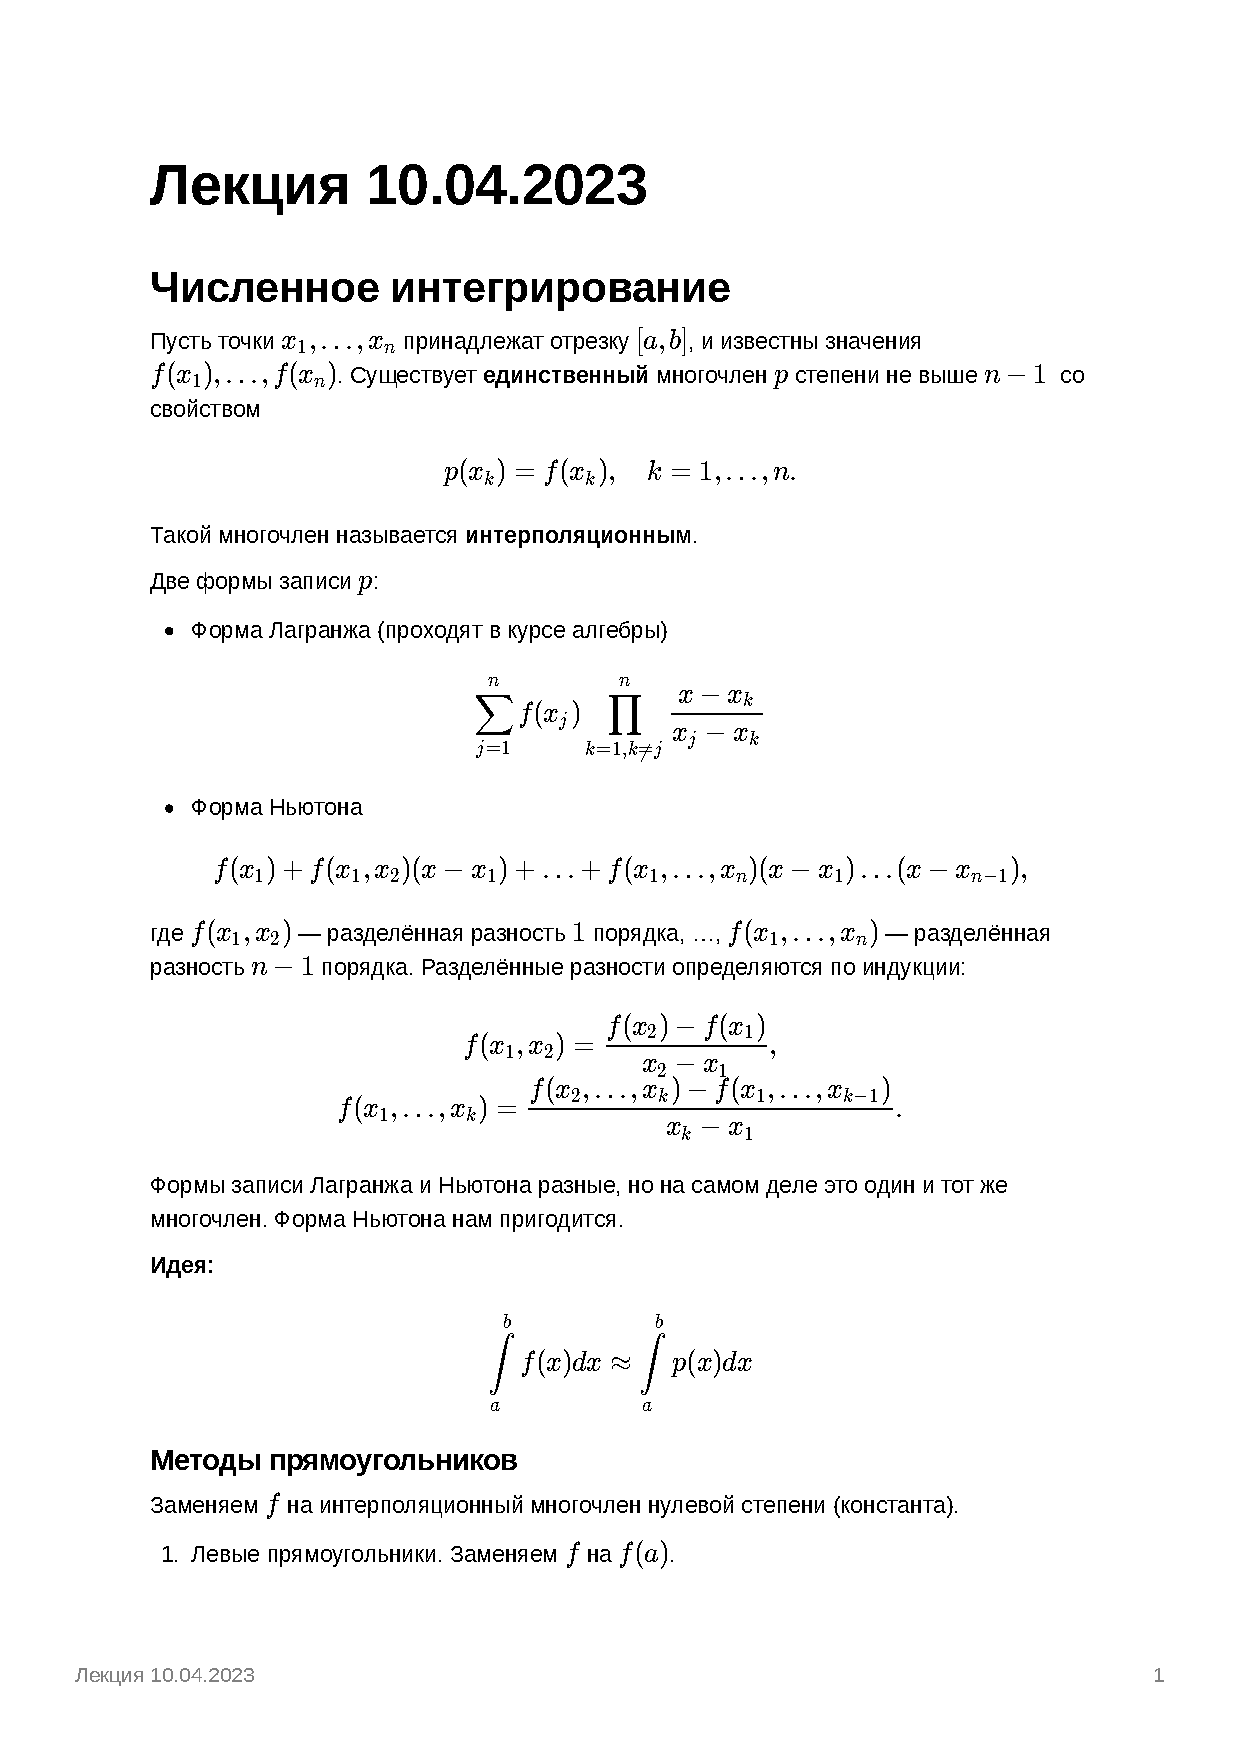
\includepdf[pages={1-}]{numerical_integrals.pdf} 


\hypertarget{tasks}{}
\section*{Несколько задач}

\subsection{$f$ непрерывна на $[a,b]$ и $\int_a^b f = 0$, $f$ знакопостоянна на $[a,b]$. Доказать, что $f(x)=0 \quad \forall x \in [a,b]$}

\textbf{Доказательство.} От противного. Пусть $\exists c \in [a,b]: \quad f(c)>0$ (б.о.о $f(c)>0$, для $f(c) < 0$ аналогично).

Так как $f$ непрерывна, то найдётся окрестность $O_{\varepsilon}(c)$ такая, что $\forall x \in O_{\varepsilon}(c) \quad f(x) > 0$. Получается, на отрезке $[c-\varepsilon, c+\varepsilon]$ $f$ положительна. 

Учитывая, что $f$ знакопостоянна, то есть в нашем случае положительна на $[a,b]$, то мы не можем <<компенсировать>> ту положительную часть под графиком на отрезке $[c-\varepsilon, c+\varepsilon]$, так как на $[a,b]$ функция неотрицательна. Тогда $\int_a^b f(x)dx > 0$. Противоречие с условием задачи доказывает требуемое.

\subsection{Пусть $|f(x)| \leq M \quad \forall x > 0, \quad \forall x > 0 \quad \exists \int_0^x f(t)dt$. Доказать, что $\Phi(x) = \int_0^x f(t)dt$ равномерно непрерывна на $[0, +\infty)$.}

\textbf{Доказательство.}
Запишем определение равномерной непрерывности для $\Phi$, которое мы хотим доказать:

\[
\forall \varepsilon > 0 \quad \exists \delta(\varepsilon) \quad \forall x' > x'' \geq 0 \quad x'-x''<\delta \Rightarrow |\Phi(x') - \Phi(x'')| < \varepsilon
\]

\[
|\Phi(x') - \Phi(x'')| = \left| \int_0^{x'} f(t)dt - \int_0^{x''} f(t)dt \right| = \left| \int_{x''}^{x'} f(t)dt \right| \leq M(x'-x'') < M\delta 
\]

Сейчас мы хотим сделать $M\delta < \varepsilon$. Поэтому сделаем $\delta < \frac{\varepsilon}{M}$

\subsection{Пусть $f$ интегрируема на $[0,1]$ и $\int_0^1 f(x)dx < 0$. Доказать, что $\exists [\alpha, \beta] \quad f \leq 0$ на $[\alpha, \beta]$.}

\textbf{Доказательство.} От противного. 
\[ \forall [\alpha, \beta] \subset [0,1] \quad \exists c \in [\alpha, \beta] \quad f(c) > 0\]

По условию 

\[ \lim_{n \rightarrow \infty} \sum_{k=1}^n f(\xi_k) \Delta x_k < 0
\]

Зафиксируем $n$. Разобъём наш отрезок $[0,1]$ на $n$ отрезочков, для каждого из которых найдём $\xi_i$ такое, что $f(\xi_i) > 0 \Rightarrow \int_0^1 f(x)dx > 0$. Противоречие. Значит существует такой отрезок, на котором $f$ неположительна.

\subsection{Докажите, что если функция $f(x)$ непрерывна на $[-1,1]$ и для каждой непрерывной на $[-1,1]$ чётной функции $g(x)$ выполняется $\int_{-1}^1 f(x)g(x)dx = 0$, то функция $f(x)$ нечётна.}

\textbf{Доказательство.} Наша $f$ представляется как 
\[
\frac{f(x)+f(-x)}{2} + \frac{f(x)-f(-x)}{2}
\]

Причём $\frac{f(x)+f(-x)}{2}$ чётная, $\frac{f(x)-f(-x)}{2}$ --- нечётная.

Возьмём $g(x) = \frac{f(x)+f(-x)}{2}$.

Тогда 

\[
\int_{-1}^1 f(x)g(x)dx = \int_{-1}^1 \frac{f(x)+f(-x)}{2} g(x) dx + \int_{-1}^1 \frac{f(x)-f(-x)}{2} g(x) dx = 
\]

\[
= \int_1^1 g(x) \cdot g(x) dx + \int_{-1}^1 \frac{f(x)-f(-x)}{2} g(x) dx = 0
\]

$\frac{f(x)-f(-x)}{2} g(x)$ --- нечётная, $g(x)\cdot g(x)$ --- чётная.

Очевидно $\int_{-1}^1 \frac{f(x)-f(-x)}{2} g(x) dx  = 0$, тогда $\int_1^1 g(x)\cdot g(x) dx = 0$, тогда $g(x) = \frac{f(x)+f(-x)}{2} = 0$, то есть чётная часть функции равна нулю. Другими словами, $f$ нечётная.

Эти задачи сильно проще, чем те, что будут на колоке.\href{https://trusting-road-174.notion.site/c5257f208f4b499e9eea3b32bd01dfdb}{Здесь} посложнее
\end{document}
